\section{Análisis del sistema}
\subsection{Hardware}
%Requisitos de la red en si, explicando lo que tendrá que haber y como deberá conectarse, sin decir todavía cómo.
\begin{itemize}
	\item \textbf{Ordenador monitor:} Contará con un sistema operativo Linux. En este caso se ha usado Debian 9 Stretch y tendrá almacenado el fichero inicial de datos, que será modificado por el resto de nodos de la red, hasta que reciba el fichero final una vez que se complete la cadena. Es el punto de inicio y final de la cadena de nodos siendo tanto el emisor del fichero inicial como el receptor del fichero final (una vez que ha sido modificado por otros nodos de la red).
	\item \textbf{Nodos:} Cada tarjeta Zybo deberá incluir una instalación de un sistema operativo Linux para facilitar la gestión de los ficheros y las comunicaciones entre los nodos. El sistema operativo, el bitstream con el IP\footnote{Intellectual Property: \url{https://www.xilinx.com/products/intellectual-property.html}.} cifrador/descifrador y la aplicación forman una imagen desarrollada en el Trabajo de Fin de Grado de Gabriel Fernando Sánchez Reina \hyperlink{3}{[3]}. Esta imagen, se clonará en las tarjetas de memoria SD incorporadas en cada tarjeta Zybo.
	
	El proceso de clonación de las tarjetas SD lo podemos ver en el apéndice \hyperlink{InstalacionLinux}{Clonación de tarjetas SD para tarjetas Zybo.}
	
	Para el mejor reconocimiento de las tarjetas Zybo en la red, cada una contará con un nombre y una IP fija como podemos ver en la Tabla \ref{Direcciones IP de las tarjetas Zybo}.
	\begin{table}[h]
		\centering
		\begin{tabular}{|c|c|}
			\hline
			\textbf{Dispositivo} & \textbf{Dirección IP} \\ \hline
			monitor & 192.168.1.10 \\ \hline
			zybo1 & 192.168.1.11 \\ \hline
			zybo2 & 192.168.1.12 \\ \hline
			zybo3 & 192.168.1.13 \\ \hline
		\end{tabular}
		\caption{Direcciones IP de las tarjetas Zybo}
		\label{Direcciones IP de las tarjetas Zybo}
	\end{table}
	\item \textbf{Switch:} Se ha usado un switch Tp-Link TL-SG1024D al que no se le ha aplicado ninguna configuración adicional.
\end{itemize}



\subsection{Software}
%Hablará de los test que habrá que diseñar y luego de los scripts que deberán automatizar el funcionamiento del sistema.
Para la transmisión del fichero de datos, usaremos SSH \hyperlink{4}{[4]} debido a que nos ofrece la mayor seguridad a la hora de enviar ficheros a través de la red.

Se han diseñado una serie de scripts para automatizar el proceso de transmisión, cifrado/descifrado y adición de datos. Estos scripts\footnote{Para ver detalladamente todos los scripts, ver el \hyperlink{Scripts}{Apéndice B}.} son los siguientes:
\begin{itemize}
	\item \hyperlink{ScriptConexion}{\textbf{\texttt{Inicio.sh}:}} Script encargado de probar las conexiones de todos los dispositivos de la red. Será lanzado manualmente desde el ordenador central para que el usuario pueda comprobar el estado de las conexiones. La ejecución de este script, será recomendado pero opcional.
	\item \hyperlink{ScriptLanzador}{\textbf{\texttt{Lanzador.sh}:}} Script encargado de lanzar el script \texttt{Automatico.sh}. Éste script será lanzado mediante la herramienta de programación de tareas \texttt{cron}.
	\item \hyperlink{ScriptAutomatico}{\textbf{\texttt{Automatico.sh}:}} Script encargado de lanzar periódicamente los siguientes scripts cada segundo. Debido a su comportamiento periódico, podemos garantizar la correcta comprobación de los directorios y ficheros implicados en el proceso.
	\begin{itemize}
		\item \hyperlink{ScriptRecibiendo}{\textbf{\texttt{Recibiendo.sh}:}} Script encargado de comprobar si se ha recibido algo y prepararlo para su tratamiento en cada nodo.
		\item \hyperlink{ScriptCristian}{\textbf{\texttt{Cristian.sh}:}} Script encargado de añadir información en cada nodo de la red. En el caso de tener implementado en hardware el IP cifrador/descifrador, será también el encargado de realizar el proceso de cifrado/descifrado a la información localmente añadida.
		\item \hyperlink{ScriptEnviando}{\textbf{\texttt{Enviando.sh}:}} Script encargado de enviar los datos al siguiente nodo. En caso de que no exista el siguiente nodo (o no esté disponible), se enviará de vuelta al ordenador central.
	\end{itemize}
	\item \hyperlink{ScriptBorrar}{\textbf{\texttt{Borrar.sh}:}} Sctipt encargado de borrar vaciar todos los directorios de trabajo. Deberá ser lanzado manualmente por el usuario en caso de querer vaciar los directorios de trabajo.
\end{itemize}

La secuencia de trabajo de estos scripts la podemos ver en la Figura \ref{Secuencia de trabajo}.
\begin{figure}[h]
	\centering
	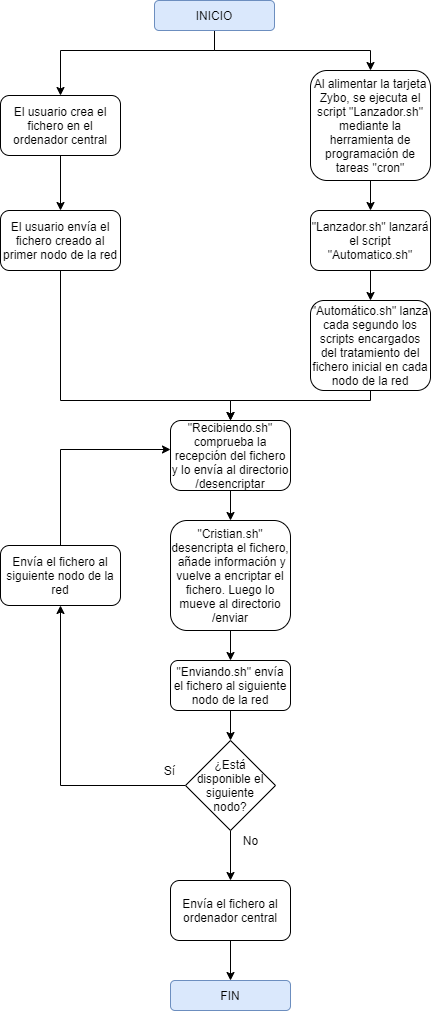
\includegraphics[scale=0.475]{Metodologia/AnalisisSistema/CadenaScripts.png}
%	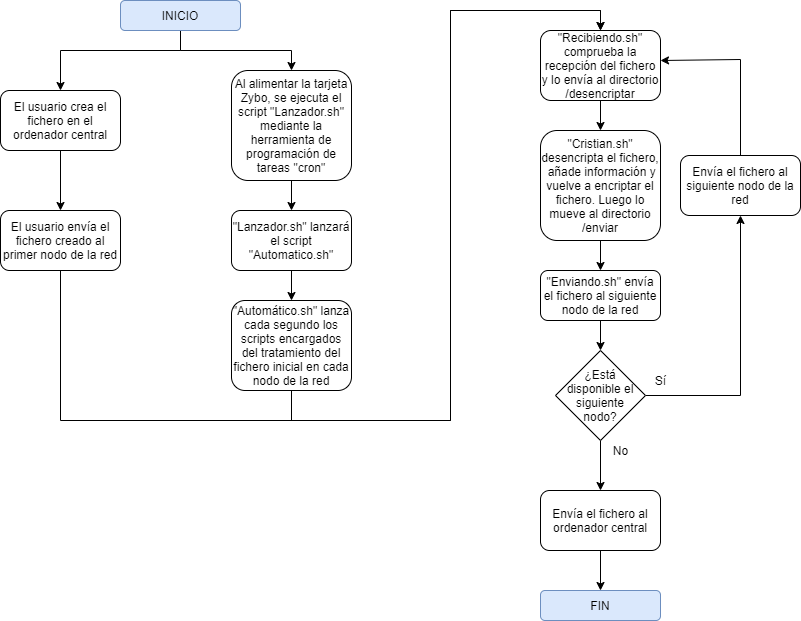
\includegraphics[scale=0.6]{Metodologia/AnalisisSistema/CadenaScriptsAncho.png}
	\caption{Secuencia de trabajo}
	\label{Secuencia de trabajo}
\end{figure}
\newpage